\documentclass[12pt]{article}
\usepackage[hidelinks]{hyperref}    
\usepackage[all]{hypcap}   
\usepackage{graphicx}
\usepackage{amsmath}
\usepackage{xcolor}
\usepackage{circuitikz}

% Define the half-adder command
\newcommand{\halfadder}[2]{
    % Inputs A and B
    % XOR Gate
    \draw
    (0, 2) node[xor port, anchor=in 1] (sum) {}
    node[anchor=east] {}
    (sum.in 2) node[anchor=east] {}
    (sum.in 1) -- ++(-2,0) node[anchor=east] {#1} -- ++(0,-2)
    (sum.in 2) -- ++(-1,0) node[anchor=east] {#2} -- ++(0,-2);

    % AND Gate
    \draw
    (0, 0) node[and port, anchor=in 1] (carry) {}
    node[anchor=east] {}
    (carry.in 2) node[anchor=east] {}
    (carry.in 1) -- ++(-2,0) node[anchor=east] {#1} -- ++(0,-1)
    (carry.in 2) -- ++(-1,0) node[anchor=east] {#2} -- ++(0,-0.5);
}

\graphicspath{{../images/}}
\author{Andrea Malvezzi}
\title{\textbf{Architettura degli Elaboratori\\ALU HACK}}
\date{09 Ottobre, 2024}
\author{Andrea Malvezzi}
\begin{document}
\maketitle
\pagebreak
\tableofcontents
\pagebreak
\section{L'architettura HACK}
L'architettura HACK si basa su un ALU che, a differenza di quella nei PC più comuni, lavora su 16 bit, senza bit di overflow (occorre quindi andare a controllare il segno dei risultati per evitare errori).\\
Questa ALU effettua operazioni su due parole da 16 bit in base al valore logico di 6 bit di controllo, per poi trasmettere su un bus di out il risultato ottenuto.
\subsection{La somma}
Per implementare la somma, oltre che alla corretta sequenza di bit di controllo, all'ALU HACK occorre un circuito integrato chiamato \textbf{Full-Adder}, realizzabile mediante \textbf{Half-Adder}.\\
In questi circuiti, l'operazione della somma viene rappresentata da una XOR, mentre il riporto dell'operazione corrisponde a una AND (si ha riporto \textit{solo} se entrambi gli input sono 1).
\subsubsection{Half-Adder}
Quindi, un half-Adder si potrà implementare nella maniera seguente:
\begin{center}
    \label{logic:half_adder}
    \begin{circuitikz}
        \halfadder{C1}{C2}
    \end{circuitikz} 
\end{center}
\pagebreak
\subsubsection{Full-Adder}
Ora, per realizzare un \textbf{Full-Adder} a 3 bit, useremo due Half-Adder e un ulteriore AND:
\begin{figure}[!htb]
    \centering
    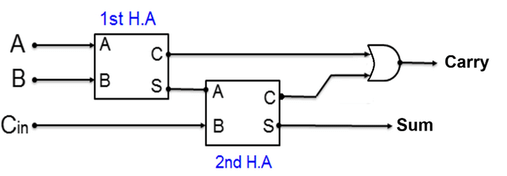
\includegraphics[width=.9\linewidth,height=.40\textheight,keepaspectratio]{ALU_HACK/full-adder.png} % essenzialmente resiza l'immagine
    \begin{center}
        \caption{\label{fig:full_adder} Esempio di Full-Adder (i rettangoli sono Half-Adder).} % label fuori da caption spesso non va, mettilo dentro
    \end{center}
\end{figure}
\end{document}